\documentclass[article]{IEEEtran}
\usepackage[brazilian]{babel}
\usepackage[utf8]{inputenc}
\usepackage{cite}
\usepackage{geometry}
\usepackage{graphicx}
\usepackage{amsmath}
\graphicspath{{./images/}}
\begin{document}

%
% paper title
% Titles are generally capitalized except for words such as a, an, and, as,
% at, but, by, for, in, nor, of, on, or, the, to and up, which are usually
% not capitalized unless they are the first or last word of the title.
% Linebreaks \\ can be used within to get better formatting as desired.
% Do not put math or special symbols in the title.
\title{Utilização de fibras óticas em sistemas de telecomunicação}



% author names and affiliations
% transmag papers use the long conference author name format.

\author{
	Felipe C. S. Santos,
	\and
	Thiago K. Lago
	
\IEEEauthorblockA{Universidade Federal do Rio de janeiro \\ 
	Escola Polit\'{e}cnica \\
	Departamento de Engenharia Eletrônica}
}



\IEEEtitleabstractindextext{
\begin{abstract}

\end{abstract}
\begin{IEEEkeywords}
Telecomunicações, fibras óticas, optoeletrônica
\end{IEEEkeywords}}



% make the title area
\maketitle

\IEEEdisplaynontitleabstractindextext
As fibras óticas tem diversas finalidades, sendo uma das mais importantes a utilização em telecomunicações. O avanço das tecnologias de fabricação, modulação e também instrumentação tem tornado cada vez mais viável a utilização das mesmas para transmissões de dados a grandes distâncias com altas taxas de bits. Busca-se através deste paper mostrar o processo de escolha de dimensionamento de uma rede baseada em componentes óticos.
\IEEEpeerreviewmaketitle



\section{Introducão}

\section{Construção da fibra}
Comentar sobre os materiais que são construídos, as janelas de transmissão, os tipos de dispersão, custo-benefício de cada uma delas.

\section{Componentes óticos}
Comentar sobre alguns componentes óticos utilizados como fbg para filtragem dos sinais e amplificadores óticos

\section{Instrumentação}
Comentar sobre os instrumentos utilizados como OTDR e espectrômetro

\section{Modulações utilizadas}
\subsection{Amplitude Shift Keying (ASK)}
\par A modulação ASK (Amplitude Shift Keying) é um tipo de modulação por intensidade do sinal da portadora, também conhecida por ON-OFF-keying. O sinal é modulado em uma portadora óptica de alta frequência. Na técnica ASK, um sinal de frequência da portadora é adicionado ao sinal da mensagem. Logo uma mensagem com o bit 1, é transmitido um sinal com A W. Enquanto que no bit 0 com 0 W. A modulação ASK é simples de gerar e detectar. No ponto de detecção, a demodulação pode ser realizada facilmente utilizando um detector fotovoltaico, que converte a energia óptica em elétrica, resultando o sinal transmitido.
\par	Para um sistema mais avançado de comunicação, é possível atingir mais de um bit transmitido por símbolo. Isto aumenta a capacidade de transmissão e é conhecido como sinalização multinível. De acordo com a equação $M = 2^N$, M representa o nível do sinal e N o número de bits por segundo e é chamado de M-ary signaling.
\begin{figure}[hb]
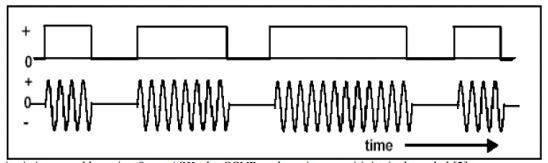
\includegraphics[width=\columnwidth]{ask.png}
\caption{Exemplo de sinal modulado com ASK}
\end{figure}

\subsection{Frequency Shift Keying (FSK)}
\par A modulação FSK é quando a freqüência do laser é trocada entre as duas freqüências. Nesta técnica de modulação. Comparando com a modulação ASK,a complexidade de gerar e receber do sistema aumenta. O formato de modulação diferente baseado no FSK pode ser definido mudando valor do índice de modulação. Uma pequena mudança no índice de modulação resulta em um espectro óptico mais compacto. Em sistemas já implantados, um formato de modulação não pode ser substituído pelo formato de modulação baseado em FSK devido à complexidade do sistema receptor. Nesta técnica, os parâmetros do transmissor e os  parâmetros do receptor devem ser idênticos.

\begin{figure}[hb]
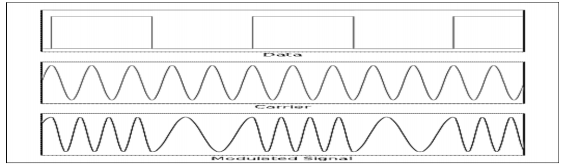
\includegraphics[width=\columnwidth]{fsk.png}
\caption{Exemplo de sinal modulado com FSK}
\end{figure}

\subsection{Phase Shift Keying (PSK)}
\par Phase Shift Keying é a técnica de modulação digital em que a fase da portadora muda, alterando a entrada por senos ou cossenos. Essa modulação possui  dois tipos, a BPSK e QPSK.
\subsubsection{BPSK}
\par Nesta técnica, a portadora senoidal toma duas formas de phase, 0º e 180º.
\subsubsection{QPSK}
\par Nesta técnica, a portadora senoidal pode tomar diversos valores de fase como 0º, 90º, 180º e 270º.

\begin{figure}[h]
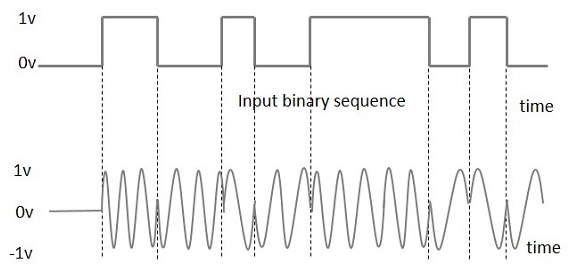
\includegraphics[width=\columnwidth]{psk.png}
\caption{Exemplo de sinal modulado com PSK}
\end{figure}

\subsection{Polarization Shift Keying (PolSK)}
Na modulação PolSK existem dois estados ortogonais de polarização entre o qual o sinal polarizado é mudado para gerar o sinal PolSK. Nesta modulação, o conteúdo do sinal é constante , o que melhora a tolerância não linear e sensibilidade para uma melhor utilização da largura de banda do sistema, a modulação PolSK possui um complexo sistema de geração e detecção de sinais, e também é muito sensível a distúrbios de polarização que podem ocorrer na linha de transmissão.
\begin{figure}[h]
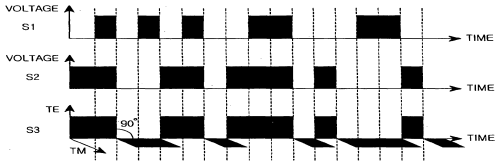
\includegraphics[width=\columnwidth]{polsk.png}
\caption{Exemplo de sinal modulado com PolSK}
\end{figure}
\section{Conclusão}



\end{document}


